% move all configuration stuff into includes file so we can focus on the content
\documentclass[aspectratio=169,hyperref={pdfpagelabels=false,colorlinks=true,linkcolor=white,urlcolor=lightblue},xcolor={table},t]{beamer}

%%%%%%%%%%%%%%%%%%%%%%%%%%%%%%%%%%%%%%%%%%%%%%%%%%%%%%%%%%%%%%%%%%%%%%%%%%%%%%%%%%
%%%%%%%%%%%%%%%%%%%%%%%%%%%%%%%%%%%%%%%%%%%%%%%%%%%%%%%%%%%%%%%%%%%%%%%%%%%%%%%%%%
% packages
\usepackage{pict2e}
\usepackage{epic}
\usepackage{amsmath,amsfonts,amssymb}
\usepackage{units}
\usepackage{fancybox}
\usepackage[absolute,overlay]{textpos} 
%\usepackage[table]{xcolor}
\usepackage{animate}
\usepackage{gensymb}
%\usepackage{graphicx}
%\usepackage{longtable}
\usepackage{multirow}
\usepackage{silence}
\usepackage{tikz}
\usepackage[backend=bibtex,style=ieee]{biblatex}
\AtEveryCitekey{\iffootnote{\tiny}{}}
\addbibresource{include/references}



% fontsize
\let\Tiny=\tiny

%%%%%%%%%%%%%%%%%%%%%%%%%%%%%%%%%%%%%%%%%%%%%%%%%%%%%%%%%%%%%%%%%%%%%%%%%%%%%%%%%%
%%%%%%%%%%%%%%%%%%%%%%%%%%%%%%%%%%%%%%%%%%%%%%%%%%%%%%%%%%%%%%%%%%%%%%%%%%%%%%%%%%
% warnings
\pdfsuppresswarningpagegroup=1
\WarningFilter{biblatex}{Patching footnotes failed}
\WarningFilter{latexfont}{Font shape}
\WarningFilter{latexfont}{Some font shapes}
\WarningFilter{gensymb}{Not defining}


%%%%%%%%%%%%%%%%%%%%%%%%%%%%%%%%%%%%%%%%%%%%%%%%%%%%%%%%%%%%%%%%%%%%%%%%%%%%%%%%%%
%%%%%%%%%%%%%%%%%%%%%%%%%%%%%%%%%%%%%%%%%%%%%%%%%%%%%%%%%%%%%%%%%%%%%%%%%%%%%%%%%%
% theme & layout
\usetheme{Frankfurt}
\useinnertheme{rectangles}


%%%%%%%%%%%%%%%%%%%%%%%%%%%%%%%%%%%%%%%%%%%%%%%%%%%%%%%%%%%%%%%%%%%%%%%%%%%%%%%%%%
\setbeamertemplate{frametitle}[default][colsep=-4bp,rounded=false,shadow=false]
\setbeamertemplate{frametitle}
{%
    \nointerlineskip%
    %\vskip-0.5ex
    \begin{beamercolorbox}[wd=\paperwidth,ht=3.5ex,dp=0.6ex]{frametitle}
        \hspace*{1.3ex}\insertframetitle%
        
        \hspace*{1.3ex}\small\insertframesubtitle%
    \end{beamercolorbox}%
    \begin{textblock*}{100mm}(13.75cm,1cm)
        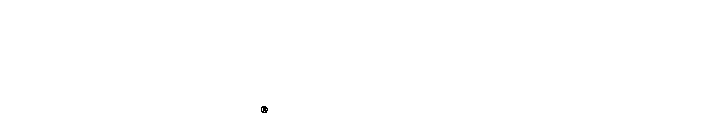
\includegraphics[height=.4cm,keepaspectratio]{graph/Logo_GTCMT_white}
    \end{textblock*}
}


%%%%%%%%%%%%%%%%%%%%%%%%%%%%%%%%%%%%%%%%%%%%%%%%%%%%%%%%%%%%%%%%%%%%%%%%%%%%%%%%%%
\setbeamertemplate{title page}[default][colsep=-4bp,rounded=false,shadow=false]
\setbeamertemplate{title page}
{
    \begin{textblock*}{100mm}(15cm,.51cm)
            \href{https://github.com/alexanderlerch/ACA-Slides/blob/2nd_edition/\jobname.pdf}{\includegraphics[height=.5cm,keepaspectratio]{graph/Logo_github}}\hspace*{2ex}
    \end{textblock*}
    \begin{textblock*}{100mm}(15cm,1.3cm)
            \href{\IEEELink}{
\includegraphics[height=.5cm,keepaspectratio]{graph/icon/book}}\hspace*{2ex}
    \end{textblock*}
    \vskip-10ex
    \begin{beamercolorbox}[wd=\paperwidth,ht=.7\paperheight,dp=0.6ex]{frametitle} %35ex
        %\begin{flushright}
            %\href{http://www.gtcmt.gatech.edu}{
\includegraphics[height=.8cm,keepaspectratio]{graph/Logo_GTCMT_black}}\hspace*{2ex}
        %\end{flushright}
        
        \hspace*{1.8ex}\LARGE\inserttitle%
        
        \vspace*{.5ex}
        
        \hspace*{1.3ex}\small\insertsubtitle%
        
        \vspace*{.5ex}
    \end{beamercolorbox}%
    \nointerlineskip%
    \begin{beamercolorbox}[wd=\paperwidth,ht=.4\paperheight,dp=0.6ex]{page number in head/foot}
        %\vspace*{-.5ex}
        \hspace*{1.7ex}\small\insertauthor%
        
        %\hspace*{1.7ex}\small }%
        
        \vspace*{12ex}
        \vfill
        \begin{flushright}
            \href{http://www.gtcmt.gatech.edu}{
\includegraphics[height=.5cm,keepaspectratio]{graph/Logo_GTCMT_black}}\hspace*{2ex}
        \end{flushright}
    \end{beamercolorbox}%
}


%%%%%%%%%%%%%%%%%%%%%%%%%%%%%%%%%%%%%%%%%%%%%%%%%%%%%%%%%%%%%%%%%%%%%%%%%%%%%%%%%%
%\makeatother
\setbeamertemplate{footline}
{
  \leavevmode%
  \hbox{%
  \begin{beamercolorbox}[wd=.5\paperwidth,ht=2.25ex,dp=1ex,left,leftskip=1ex]{page number in head/foot}%
    \insertsubtitle
  \end{beamercolorbox}%
  \begin{beamercolorbox}[wd=.5\paperwidth,ht=2.25ex,dp=1ex,right,rightskip=1ex]{page number in head/foot}%
    \hfill
    \insertframenumber{} / \inserttotalframenumber
  \end{beamercolorbox}}%
  \vskip0pt%
}
%\makeatletter


%%%%%%%%%%%%%%%%%%%%%%%%%%%%%%%%%%%%%%%%%%%%%%%%%%%%%%%%%%%%%%%%%%%%%%%%%%%%%%%%%%
\beamertemplatenavigationsymbolsempty
\setbeamertemplate{navigation symbols}{}
\setbeamertemplate{blocks}[default]%[rounded=false,shadow=false]
\setbeamertemplate{itemize item}[square]
\setbeamertemplate{itemize subitem}[circle]
\setbeamertemplate{itemize subsubitem}[triangle]
\setbeamertemplate{enumerate item}[square]
\setbeamertemplate{enumerate subitem}[circle]
\setbeamertemplate{enumerate subsubitem}[circle]


%%%%%%%%%%%%%%%%%%%%%%%%%%%%%%%%%%%%%%%%%%%%%%%%%%%%%%%%%%%%%%%%%%%%%%%%%%%%%%%%%%
% colors
\setbeamercolor{structure}{fg=darkgray}
\setbeamercovered{transparent} %invisible
\setbeamercolor{bibliography entry author}{fg=black}
\setbeamercolor*{bibliography entry title}{fg=black}
\setbeamercolor*{bibliography entry note}{fg=black}
\setbeamercolor{frametitle}{fg=black}
\setbeamercolor{title}{fg=white}
\setbeamercolor{subtitle}{fg=white}
\setbeamercolor{frametitle}{fg=white}
\setbeamercolor{framesubtitle}{fg=white}
\setbeamercolor{mini frame}{fg=white, bg=black}
\setbeamercolor{section in head/foot}{fg=white, bg=darkgray}
\setbeamercolor{page number in head/foot}{fg=black, bg=lightblue}
\setbeamercolor{item projected}{fg=white, bg=black}

%---------------------------------------------------------------------------------
%%%%%%%%%%%%%%%%%%%%%%%%%%%%%%%%%%%%%%%%%%%%%%%%%%%%%%%%%%%%%%%%%%%%%%%%%%%%%%%%%%
%%%%%%%%%%%%%%%%%%%%%%%%%%%%%%%%%%%%%%%%%%%%%%%%%%%%%%%%%%%%%%%%%%%%%%%%%%%%%%%%%%
% title information
\title[]{Introduction to \textbf{Audio Content Analysis}}   
\author[alexander lerch]{alexander lerch} 
%\institute{~}
%\date[Alexander Lerch]{}
%\titlegraphic{\vspace{-16mm}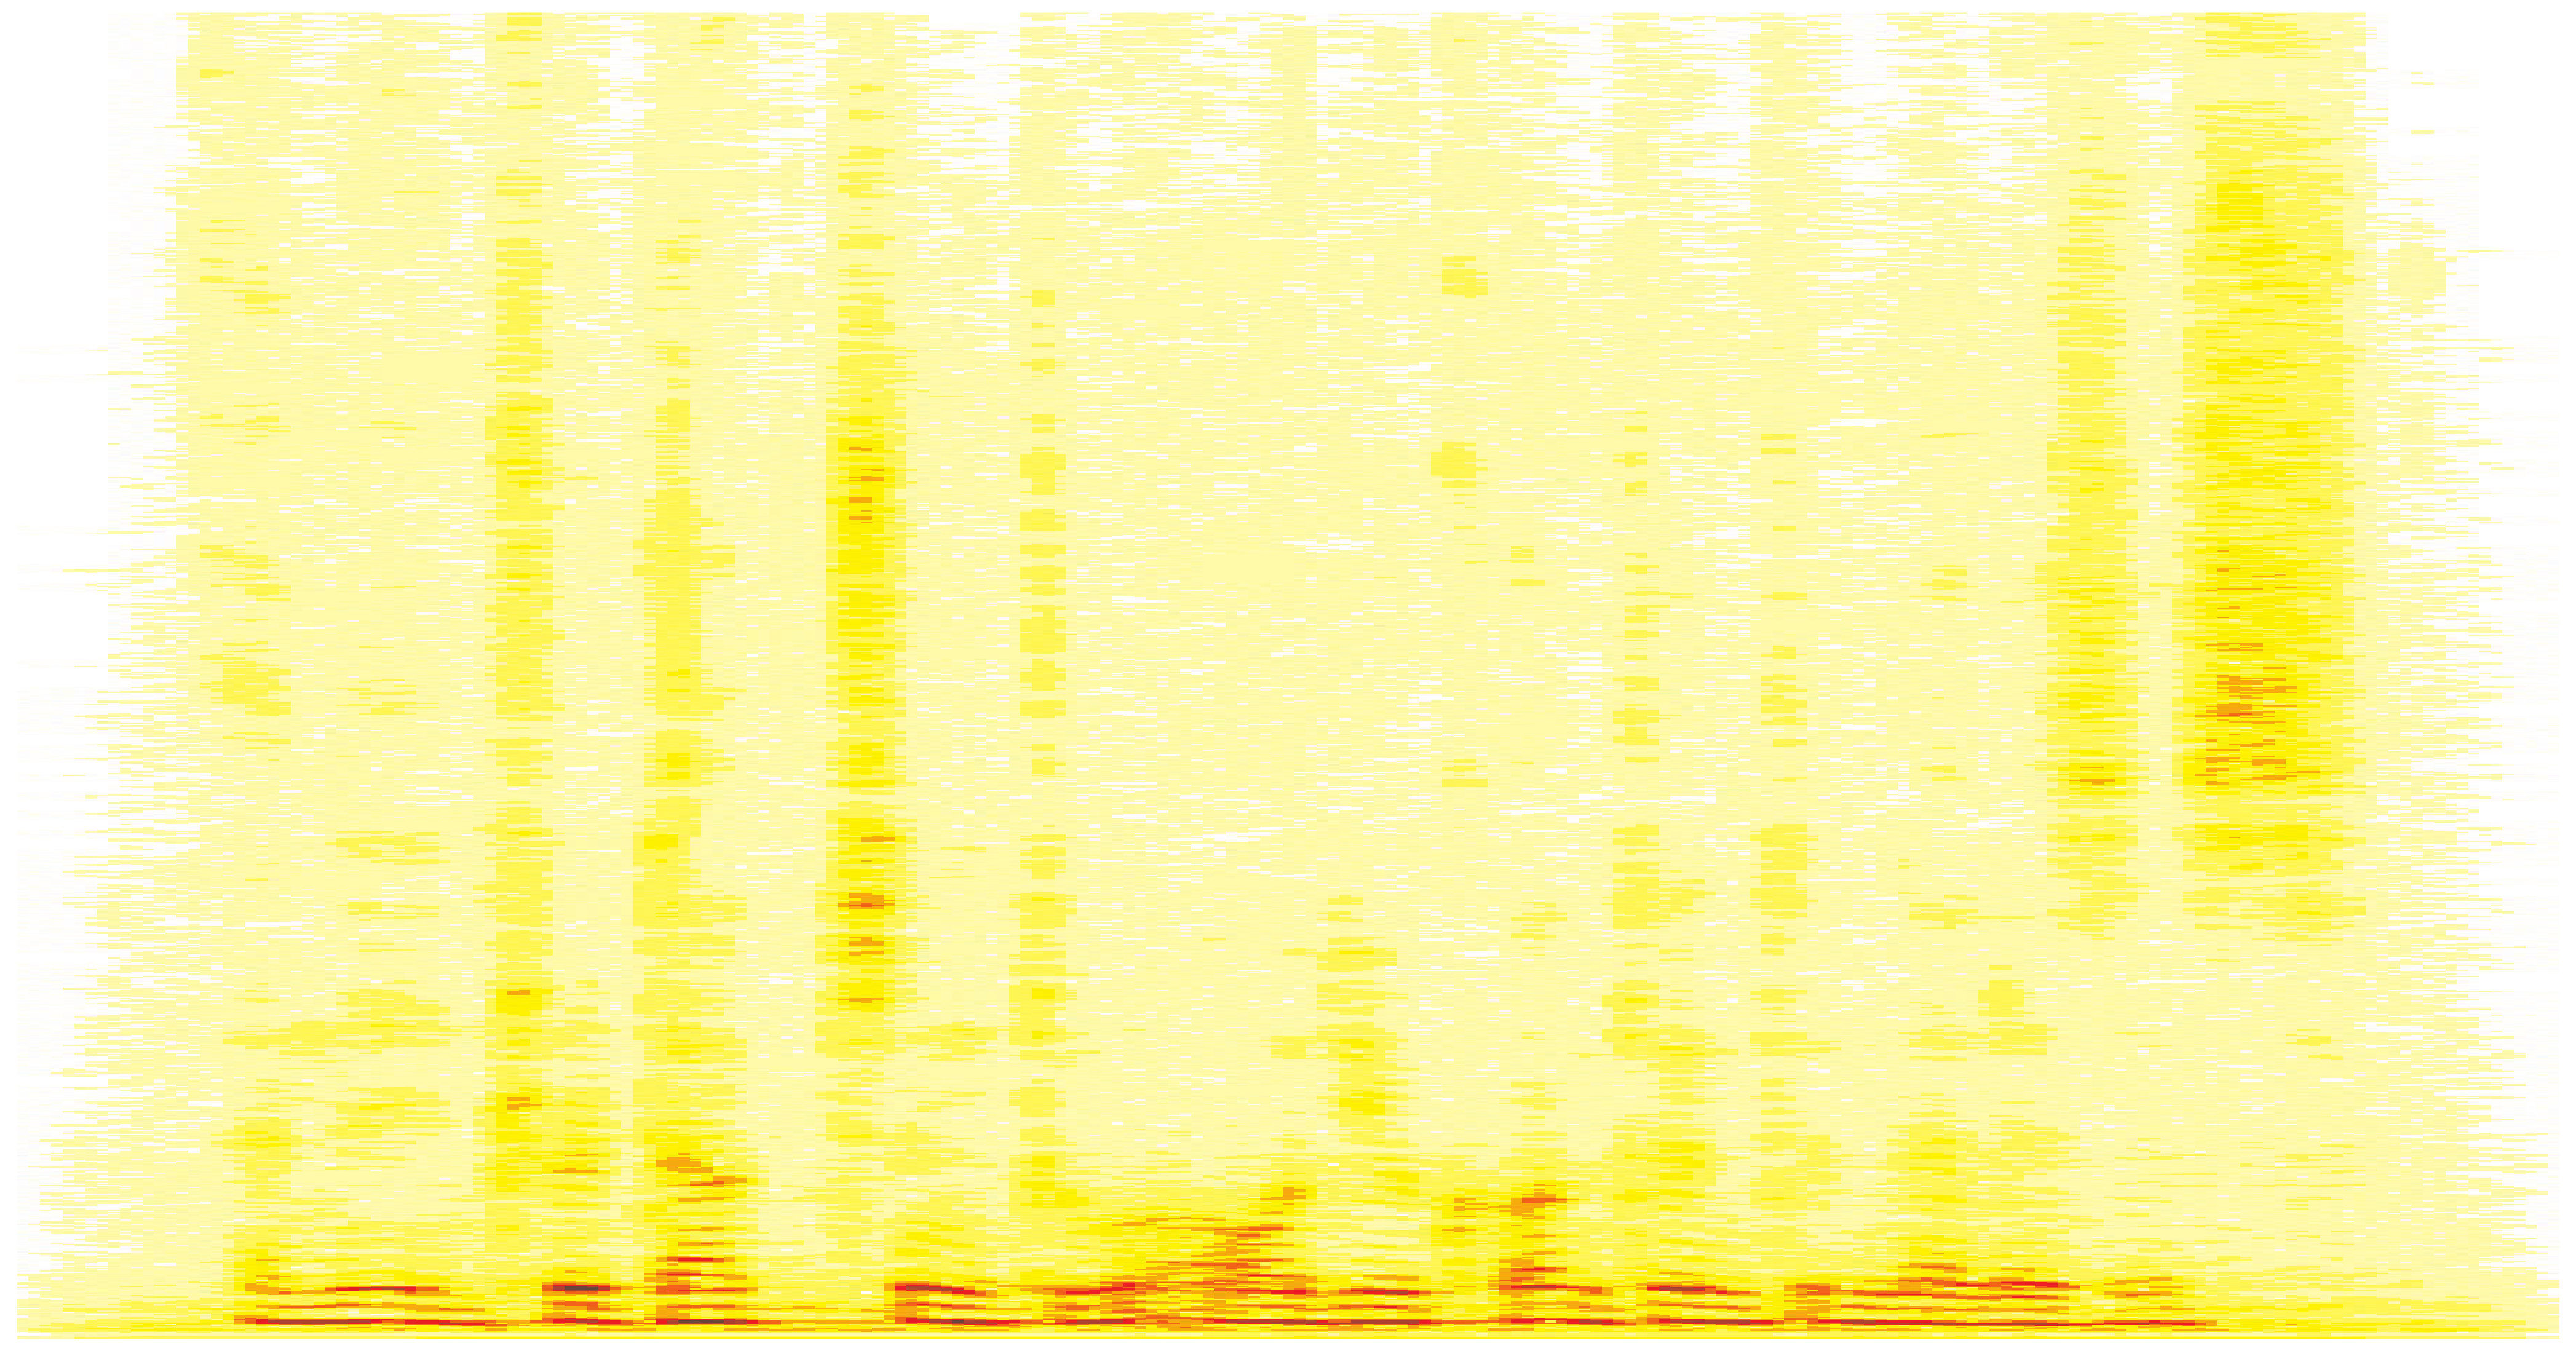
\includegraphics[width=\textwidth,height=3cm]{title}}

%%%%%%%%%%%%%%%%%%%%%%%%%%%%%%%%%%%%%%%%%%%%%%%%%%%%%%%%%%%%%%%%%%%%%%%%%%%%%%%%%%
%%%%%%%%%%%%%%%%%%%%%%%%%%%%%%%%%%%%%%%%%%%%%%%%%%%%%%%%%%%%%%%%%%%%%%%%%%%%%%%%%%
% colors
\definecolor{gtgold}{HTML}{96caff} %0e7eed {rgb}{0.88,0.66,1,0.06} [234, 170, 0]/256
\definecolor{darkgray}{rgb}{.1, .1, .25}
\definecolor{lightblue}{HTML}{0e7eed}
\definecolor{highlight}{rgb}{0, 0, 1} %_less!40

%%%%%%%%%%%%%%%%%%%%%%%%%%%%%%%%%%%%%%%%%%%%%%%%%%%%%%%%%%%%%%%%%%%%%%%%%%%%%%%%%%
%%%%%%%%%%%%%%%%%%%%%%%%%%%%%%%%%%%%%%%%%%%%%%%%%%%%%%%%%%%%%%%%%%%%%%%%%%%%%%%%%%
% relative paths
\graphicspath{{../ACA-Plots/graph/}}


%%%%%%%%%%%%%%%%%%%%%%%%%%%%%%%%%%%%%%%%%%%%%%%%%%%%%%%%%%%%%%%%%%%%%%%%%%%%%%%%%%
%%%%%%%%%%%%%%%%%%%%%%%%%%%%%%%%%%%%%%%%%%%%%%%%%%%%%%%%%%%%%%%%%%%%%%%%%%%%%%%%%%
% units
\setlength{\unitlength}{1mm}

%%%%%%%%%%%%%%%%%%%%%%%%%%%%%%%%%%%%%%%%%%%%%%%%%%%%%%%%%%%%%%%%%%%%%%%%%%%%%%%%%%
%%%%%%%%%%%%%%%%%%%%%%%%%%%%%%%%%%%%%%%%%%%%%%%%%%%%%%%%%%%%%%%%%%%%%%%%%%%%%%%%%%
% math
\DeclareMathOperator*{\argmax}{argmax}
\DeclareMathOperator*{\argmin}{argmin}
\DeclareMathOperator*{\atan}{atan}
\DeclareMathOperator*{\arcsinh}{arcsinh}
\DeclareMathOperator*{\sign}{sign}
\DeclareMathOperator*{\tcdf}{tcdf}
\DeclareMathOperator*{\si}{sinc}
\DeclareMathOperator*{\princarg}{princarg}
\DeclareMathOperator*{\arccosh}{arccosh}
\DeclareMathOperator*{\hwr}{HWR}
\DeclareMathOperator*{\flip}{flip}
\DeclareMathOperator*{\sinc}{sinc}
\DeclareMathOperator*{\floor}{floor}
\newcommand{\e}{{e}}
\newcommand{\jom}{\mathrm{j}\omega}
\newcommand{\jOm}{\mathrm{j}\Omega}
\newcommand   {\mat}[1]    		{\boldsymbol{\uppercase{#1}}}		%bold
\renewcommand {\vec}[1]    		{\boldsymbol{\lowercase{#1}}}		%bold

%%%%%%%%%%%%%%%%%%%%%%%%%%%%%%%%%%%%%%%%%%%%%%%%%%%%%%%%%%%%%%%%%%%%%%%%%%%%%%%%%%
%%%%%%%%%%%%%%%%%%%%%%%%%%%%%%%%%%%%%%%%%%%%%%%%%%%%%%%%%%%%%%%%%%%%%%%%%%%%%%%%%%
% media9
\newcommand{\includeaudio}[1]{
\href{run:audio/#1.mp3}{
\includegraphics[width=5mm, height=5mm]{graph/SpeakerIcon}}}

\newcommand{\includeanimation}[4]{{\begin{center}
                        \animategraphics[autoplay,loop,scale=.7]{#4}{animation/#1-}{#2}{#3}        
                        \end{center}
                        \addreference{matlab source: \href{https://github.com/alexanderlerch/ACA-Plots/blob/master/matlab/animate#1.m}{matlab/animate#1.m}}}
                        \inserticon{video}}
                        
%%%%%%%%%%%%%%%%%%%%%%%%%%%%%%%%%%%%%%%%%%%%%%%%%%%%%%%%%%%%%%%%%%%%%%%%%%%%%%%%%%
%%%%%%%%%%%%%%%%%%%%%%%%%%%%%%%%%%%%%%%%%%%%%%%%%%%%%%%%%%%%%%%%%%%%%%%%%%%%%%%%%%
% other commands
\newcommand{\question}[1]{%\vspace{-4mm}
                          \setbeamercovered{invisible}
                          \begin{columns}[T]
                            \column{.9\textwidth}
                                \textbf{#1}
                            \column{.1\textwidth}
                                \vspace{-8mm}
                                \begin{flushright}
                                     
\includegraphics[width=.9\columnwidth]{graph/question_mark}
                                \end{flushright}
                                \vspace{6mm}
                          \end{columns}\pause\vspace{-12mm}}

\newcommand{\toremember}[1]{
                        \inserticon{lightbulb}
                        }

\newcommand{\matlabexercise}[1]{%\vspace{-4mm}
                          \setbeamercovered{invisible}
                          \begin{columns}[T]
                            \column{.8\textwidth}
                                \textbf{matlab exercise}: #1
                            \column{.2\textwidth}
                                \begin{flushright}
                                     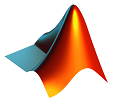
\includegraphics[scale=.5]{graph/logo_matlab}
                                \end{flushright}
                                %\vspace{6mm}
                          \end{columns}}

\newcommand{\addreference}[1]{  
                  
                    \begin{textblock*}{\baselineskip }(.98\paperwidth,.5\textheight) %(1.15\textwidth,.4\textheight)
                         \begin{minipage}[b][.5\paperheight][b]{1cm}%
                            \vfill%
                             \rotatebox{90}{\tiny {#1}}
                        \end{minipage}
                   \end{textblock*}
                    }
                    
\newcommand{\figwithmatlab}[1]{
                    \begin{figure}
                        \centering
                        \includegraphics[scale=.7]{#1}
                        %\label{fig:#1}
                    \end{figure}
                    
                    \addreference{matlab source: \href{https://github.com/alexanderlerch/ACA-Plots/blob/main/matlab/plot#1.m}{plot#1.m}}}
\newcommand{\figwithref}[2]{
                    \begin{figure}
                        \centering
                        \includegraphics[scale=.7]{#1}
                        \label{fig:#1}
                    \end{figure}
                    
                    \addreference{#2}}  
                                    
\newcommand{\inserticon}[1]{
                    \begin{textblock*}{100mm}(14.5cm,7.5cm)
                        \includegraphics[height=.8cm,keepaspectratio]{graph/#1}
                    \end{textblock*}}            

%%%%%%%%%%%%%%%%%%%%%%%%%%%%%%%%%%%%%%%%%%%%%%%%%%%%%%%%%%%%%%%%%%%%%%%%%%%%%%%%%%
%%%%%%%%%%%%%%%%%%%%%%%%%%%%%%%%%%%%%%%%%%%%%%%%%%%%%%%%%%%%%%%%%%%%%%%%%%%%%%%%%%
% counters
\newcounter{i}
\newcounter{j}
\newcounter{iXOffset}
\newcounter{iYOffset}
\newcounter{iXBlockSize}
\newcounter{iYBlockSize}
\newcounter{iYBlockSizeDiv2}
\newcounter{iXBlockSizeDiv2}
\newcounter{iDistance}

\newcommand{\IEEELink}{https://ieeexplore.ieee.org/servlet/opac?bknumber=9965970}




\subtitle{module 9.7: music structure detection}

%%%%%%%%%%%%%%%%%%%%%%%%%%%%%%%%%%%%%%%%%%%%%%%%%%%%%%%%%%%%%%%%%%%%%%%%%%%%
\begin{document}
    % generate title page
	{
\setbeamertemplate{headline}{} 
\setbeamertemplate{footline}{} 
\begin{frame}
    \titlepage
    %\vspace{-5mm}
\end{frame}
}
\addtocounter{framenumber}{-1}


    \section[overview]{lecture overview}
        \begin{frame}{introduction}{overview}
            \begin{block}{corresponding textbook section}
                    %\href{http://ieeexplore.ieee.org/xpl/articleDetails.jsp?arnumber=6331122}{missing in textbook} 
                    section~9.7
            \end{block}

            \begin{itemize}
                \item   \textbf{lecture content}
                    \begin{itemize}
                        \item   structure in music
                        \item   self similarity and self distance matrices
                        \item   structure detection approaches
                    \end{itemize}
                \bigskip
                \item<2->   \textbf{learning objectives}
                    \begin{itemize}
                        \item   summarize basic difficulties in ground truth annotations of musical structure
                        \item   explain and interpret self similarity and self distance matrices
                        \item   summarize three domains for approaching music structure detection
                    \end{itemize}
            \end{itemize}
            \inserticon{directions}
        \end{frame}

    \section[intro]{introduction}
        \begin{frame}{music structure}{introduction}
            \begin{itemize}
                \item   \textbf{music is inherently formal}/organized/structural
                \smallskip
                \item<1->   various \textbf{hierarchical structural levels}
                    \begin{itemize}
                        \item   \textit{groups of notes} build rhythmic/melodic/harmonic patterns
                        \item   \textit{measures} group multiple events
                        \item   \textit{phrases} group several measures
                        \item   \textit{sections} contain several phrases
                        \item   several sections can comprise \textit{piece/movement}
                        \item   \ldots
                    \end{itemize}
                \smallskip
                \item<2->    \textbf{grouping} of musical elements/patterns is influenced by
                    \begin{enumerate}
                        \item   \textit{contrasts \& novelty}
                            \begin{itemize}
                                \item   rhythmic, harmonic, melodic patterns
                            \end{itemize}
                        \item   \textit{similarity and repetitions}
                            \begin{itemize}
                                \item   rhythmic, harmonic, melodic patterns
                            \end{itemize}
                        \item   \textit{homogeneity} within a section 
                            \begin{itemize}
                                \item   instrumentation, tempo, harmony
                            \end{itemize}
                    \end{enumerate}
            \end{itemize}
        \end{frame}
        \begin{frame}{music structure analysis}{introduction}
            \begin{itemize}
                \item   \textbf{objective}
                    \begin{itemize}
                        \item   reveal structural properties and relationships
                        \item   generate a list of parts and repetitions
                    \end{itemize}
                \bigskip
                \item   typical \textbf{processing steps}
                    \begin{enumerate}
                        \item   \textit{feature} extraction
                        \smallskip
                        \item   Self Distance Matrix (SDM) or \textit{Self Similarity Matrix (SSM)} computation
                        \smallskip
                        \item   \textit{segment} detection based on
                            \begin{itemize}
                                \item novelty
                                \item homogeneity
                                \item repetition
                            \end{itemize}
                    \end{enumerate}
            \end{itemize}
        \end{frame}
        \begin{frame}{music structure analysis}{example}
            {\flushright{\includeaudio{structure_example_1}}}
             \figwithmatlab{Structure}
        \end{frame}
    
    \section[ssm]{self similarity matrix}
        \begin{frame}{music structure analysis}{features 1/2}
            \begin{itemize}
                \item   features from \textbf{all categories} can have impact on structure
                    \begin{itemize}
                        \item   timbre
                            \begin{itemize}
                                \item   instrumentation, playing technique, effects, \ldots
                            \end{itemize}
                        \item   tonal content
                            \begin{itemize}
                                \item   melodic and harmonic patterns, range, \ldots
                            \end{itemize}
                        \item   rhythm content
                            \begin{itemize}
                                \item   tempo, rhythmic patterns, \ldots
                            \end{itemize}
                        \item   dynamics
                            \begin{itemize}
                                \item   loudness, range, \ldots
                            \end{itemize}
                    \end{itemize}
               \bigskip
               \item<1->    \textbf{feature aggregation}
                \begin{itemize}
                    \item   use texture window, or
                    \item   aggregate features per beat or downbeat
                \end{itemize}
            \end{itemize}
        \end{frame}
        %\begin{frame}{music structure analysis}{features 2/2}
            %\vspace{-4mm}
            %\only<1>{\figwithref{StructureFeatures_0}{matlab source: \href{https://github.com/alexanderlerch/ACA-Slides/blob/master/matlab/displayStructureFeatures.m}{matlab/displayStructureFeatures.m}}}
            %\only<2>{\figwithref{StructureFeatures_1}{matlab source: \href{https://github.com/alexanderlerch/ACA-Slides/blob/master/matlab/displayStructureFeatures.m}{matlab/displayStructureFeatures.m}}}
        %\end{frame} 
        \begin{frame}{music structure analysis}{self similarity matrix}
            \vspace{-2mm}
            \begin{equation*}
                S(n_\mathrm{A}, n_\mathrm{B}) = \mathrm{s}\big(v(n_\mathrm{A}),v(n_\mathrm{B})\big)
            \end{equation*}
            \includeaudio{bad}\vspace{-5mm}
            \figwithmatlab{Ssm}
            
        \end{frame}
        \begin{frame}{music structure analysis}{feature dependency of similarity}
            \figwithmatlab{SsmFeatures}
            Features (left to right): Pitch Chroma, RMS, MFCCs, Mel Spectrogram
        \end{frame}
    \section[novelty]{novelty analysis}
        \begin{frame}{music structure analysis}{novelty analysis}
            \begin{columns}
            \column{.3\linewidth}
                \figwithmatlab{CheckerBoard}
            \column{.7\linewidth}
                \figwithmatlab{SsmNovelty}
            \end{columns}
        \end{frame}
    \section[homogeneity]{homogeneity analysis}
        \begin{frame}{music structure analysis}{homogeneity analysis 1/2}
            \figwithmatlab{SsmLowPass}
        \end{frame}
        
        \begin{frame}{music structure analysis}{homogeneity analysis 2/2}
            \begin{itemize}
                \item   can also be used as post-processing step after novelty-based approach, e.g.
                    \begin{enumerate}
                        \item   describe each segment with features
                        \item   cluster and see which segments are grouped together
                    \end{enumerate}
            \end{itemize}
        \end{frame}
        
    \section[repetition]{repetition analysis}%\href{https://github.com/alexanderlerch/ACA-Slides/blob/master/matlab/displaySdlm.m}{matlab/displaySdlm.m}
        \begin{frame}{music structure analysis}{repetition analysis 1/2}
            \figwithmatlab{SsmRotated}
        \end{frame}
        \begin{frame}{music structure analysis}{repetition analysis 2/2}
            \begin{itemize}
                \item   while in many cases it 'looks' easy, automatic extraction is \textbf{error-prone}
                \bigskip
                \item<2->[$\Rightarrow$]   typical approaches for \textbf{enhancing} the distance/similarity/lag matrix
                    \begin{itemize}
                        \item   filtering (low pass smoothing, high pass edge detection)
                        \item   use matrices with different time resolutions
                        \item   image processing methods (e.g., erosion \& dilation)
                        \item   thresholding
                        \item   ``path search'' through probability matrix
                    \end{itemize}
            \end{itemize}
        \end{frame}
        
    \section[eval]{evaluation}
        \begin{frame}{music structure analysis}{evaluation}
            \begin{itemize}
                \item   evaluation of structure detection \textbf{challenging}
                    \begin{itemize}
                        \item   \textit{ground truth}
                            \begin{itemize}
                                \item   structure itself may be ambiguous
                                \item   depending on annotator, varying hierarchical level of labels, e.g.
                            \end{itemize}
                    \end{itemize}
                    \begin{table}
                        \centering
                        \footnotesize
                            \begin{tabular}{l|c|c|c|c|c|c|c|c|c|c|}
                                    \hline
                                  \textbf{ann 1} & intro & \multicolumn{4}{c|}{A} & \multicolumn{4}{c|}{A} & outro\\ \hline
                                  \textbf{ann 2} & intro & \multicolumn{2}{c|}{verse} & \multicolumn{2}{c|}{chorus} & \multicolumn{2}{c|}{verse} & \multicolumn{2}{c|}{chorus} & outro\\ \hline
                                  \textbf{ann 3} & intro & V$_1$ & V$_2$ & C$_1$ &C$_2$ &  V$_1$ & V$_2$ & C$_1$ &C$_2$ & outro\\
                                    \hline
                            \end{tabular}
                    \end{table}
                \bigskip
                \item<2->   \textit{method and metric}
                    \begin{itemize}
                        \item   boundary matching
                        \item   frame level, e.g., pairwise match
                    \end{itemize}
                \bigskip
                \item<3->   typical range of results
                    \begin{itemize}
                        \item   $F = 50\ldots 70\% $
                    \end{itemize}
            \end{itemize}
        \end{frame}
    
    \section{summary}
        \begin{frame}{summary}{lecture content}
            \begin{itemize}
                \item   \textbf{self similarity/distance matrices}
                    \begin{itemize}
                        \item   shows pairwise similarities/distances
                        \item   depends on input features
                    \end{itemize}
                \bigskip
                \item   \textbf{structure detection}
                    \begin{enumerate}
                        \item   novelty
                        \item   homogeneity
                        \item   repetitions
                    \end{enumerate}
            \end{itemize}
            \inserticon{summary}
        \end{frame}
\end{document}
